\documentclass[reprint,amsmath, amsfonts, amssymb, aps, letterpaper]{revtex4-1}

\usepackage{graphicx,float}
%\usepackage[caption=false]{subfig}
\usepackage{dcolumn}
\usepackage{bm}
\usepackage{enumitem}
\usepackage{tabularx}
\setlength{\extrarowheight}{6 pt}
\newcolumntype{Y}{>{\centering\arraybackslash}X}
\setlist[enumerate]{topsep=0pt,itemsep=-1ex,partopsep=1ex,parsep=1ex}
\usepackage{natbib}
\usepackage{physics}
\usepackage{fancyhdr}
\usepackage{amsthm}
\usepackage{amsmath}
\usepackage{graphicx}
\usepackage{amssymb}
\usepackage{esint}
\usepackage{color}
\usepackage{moreverb}
\usepackage{wrapfig}
\usepackage{physics}
\usepackage{siunitx}
\usepackage{subfig}
%\usepackage{wrapfig}


\begin{document}

\preprint{PHYS CS 15C}
\title{Remotely Operated Vehicle (ROV) with Touch Sensing Control}
\author{Menghang (David) Wang, Weiheng (Frank) Fu, Yiluo Li}
\affiliation{University of California, Santa Barbara, California 93107}

\date{\today}

% Intrigue your audience, connect your project with something people feel more interested in general

% to measure the systematic error, you can try best to maximize the potential one and see if it will genuinely have much effect

\begin{abstract}
<<<<<<< HEAD
Often times there exist terrain on which people cannot tread on. Whether it be disaster debris or remote terrain such as Mars, it would provide much convenience if we are allowed to control the vehicle remotely while still being able to see directly how the terrain looks like. However, current touch input technologies are better suited for flat and relative small surfaces. In 2017, Yang \citep{electrick} proposed a sensing technique that utilizes electric field tomography. Inspired by Yang, we implemented this technique in a possible realistic situation using dynamic pressure sensing instead. We successfully acquired touch input from a cardboard using machine learning, and commanded a Remote Operated Vehicle (ROV) to move to the corresponding position. This model can be easily generalized. Suppose we have a complex terrain and human is not fit for the mission, we can 3D print the terrain and guide robot to desired location with a swipe of finger. Not only is this control more intuitive, it can also provide helpful information that can aid the mission.
=======
Current touch input technologies are better suited for flat and relative small surfaces. In 2017, Yang \citep{electrick} proposed a sensing technique that utilizes electric field tomography. Inspired by Yang, we implemented this technique in a possible realistic situation using dynamic pressure sensing instead. We successfully acquired touch input from a cardboard using machine learning, and commanded a Remote Operated Vehicle (ROV) to move to the corresponding position. This model can be easily generalized. Suppose we have a complex terrain and human is not fit for the mission, we can 3D print the terrain and guide robot to desired location with a swipe of finger. Not only is this control more intuitive, it can also provide helpful information that can aid the mission.
>>>>>>> 6a97dfacc2d896add2eb77cacbc644a151c0d400
\end{abstract}

\maketitle

\section{Introduction}
Remotedly operated vehicles are already very common in performing jobs that human are not suited for, such as underwater construction, extraterrestrial exploration, work in hideous environment, and etc. However, in those situations, the robot is often monitored by multiple mounted cameras, and controlled by using a computer screen with visuals sent back from the robot. It would be hard for people in control to fully grasp the bigger map of the robot's moving zone, and it poses difficulties to evaluate the overall conditions of the terrain with just cameras. Under such circumstance, we propose to construct a robot that will follow our command on a model terrain that replicate the scale and feature of the actual terrain, as a visual aid and new way of controlling the robot directly.
\\\indent To achieve such goal, we chose to create a touching pad sprayed with carbon conductive material, and scaled the size according to the dimension of the track on which our vehicle would be walking on. This served as our toy model for the remotely controlled vehicle on a visualized terrain. On the touching pad, we used electric sensing mechanism to measure the voltage drop across different locations, process the data to predict the finger location, and send the corresponding command through infrared to the vehicle.

\subsection{Setup overview}
\begin{figure}[h]
\centering
    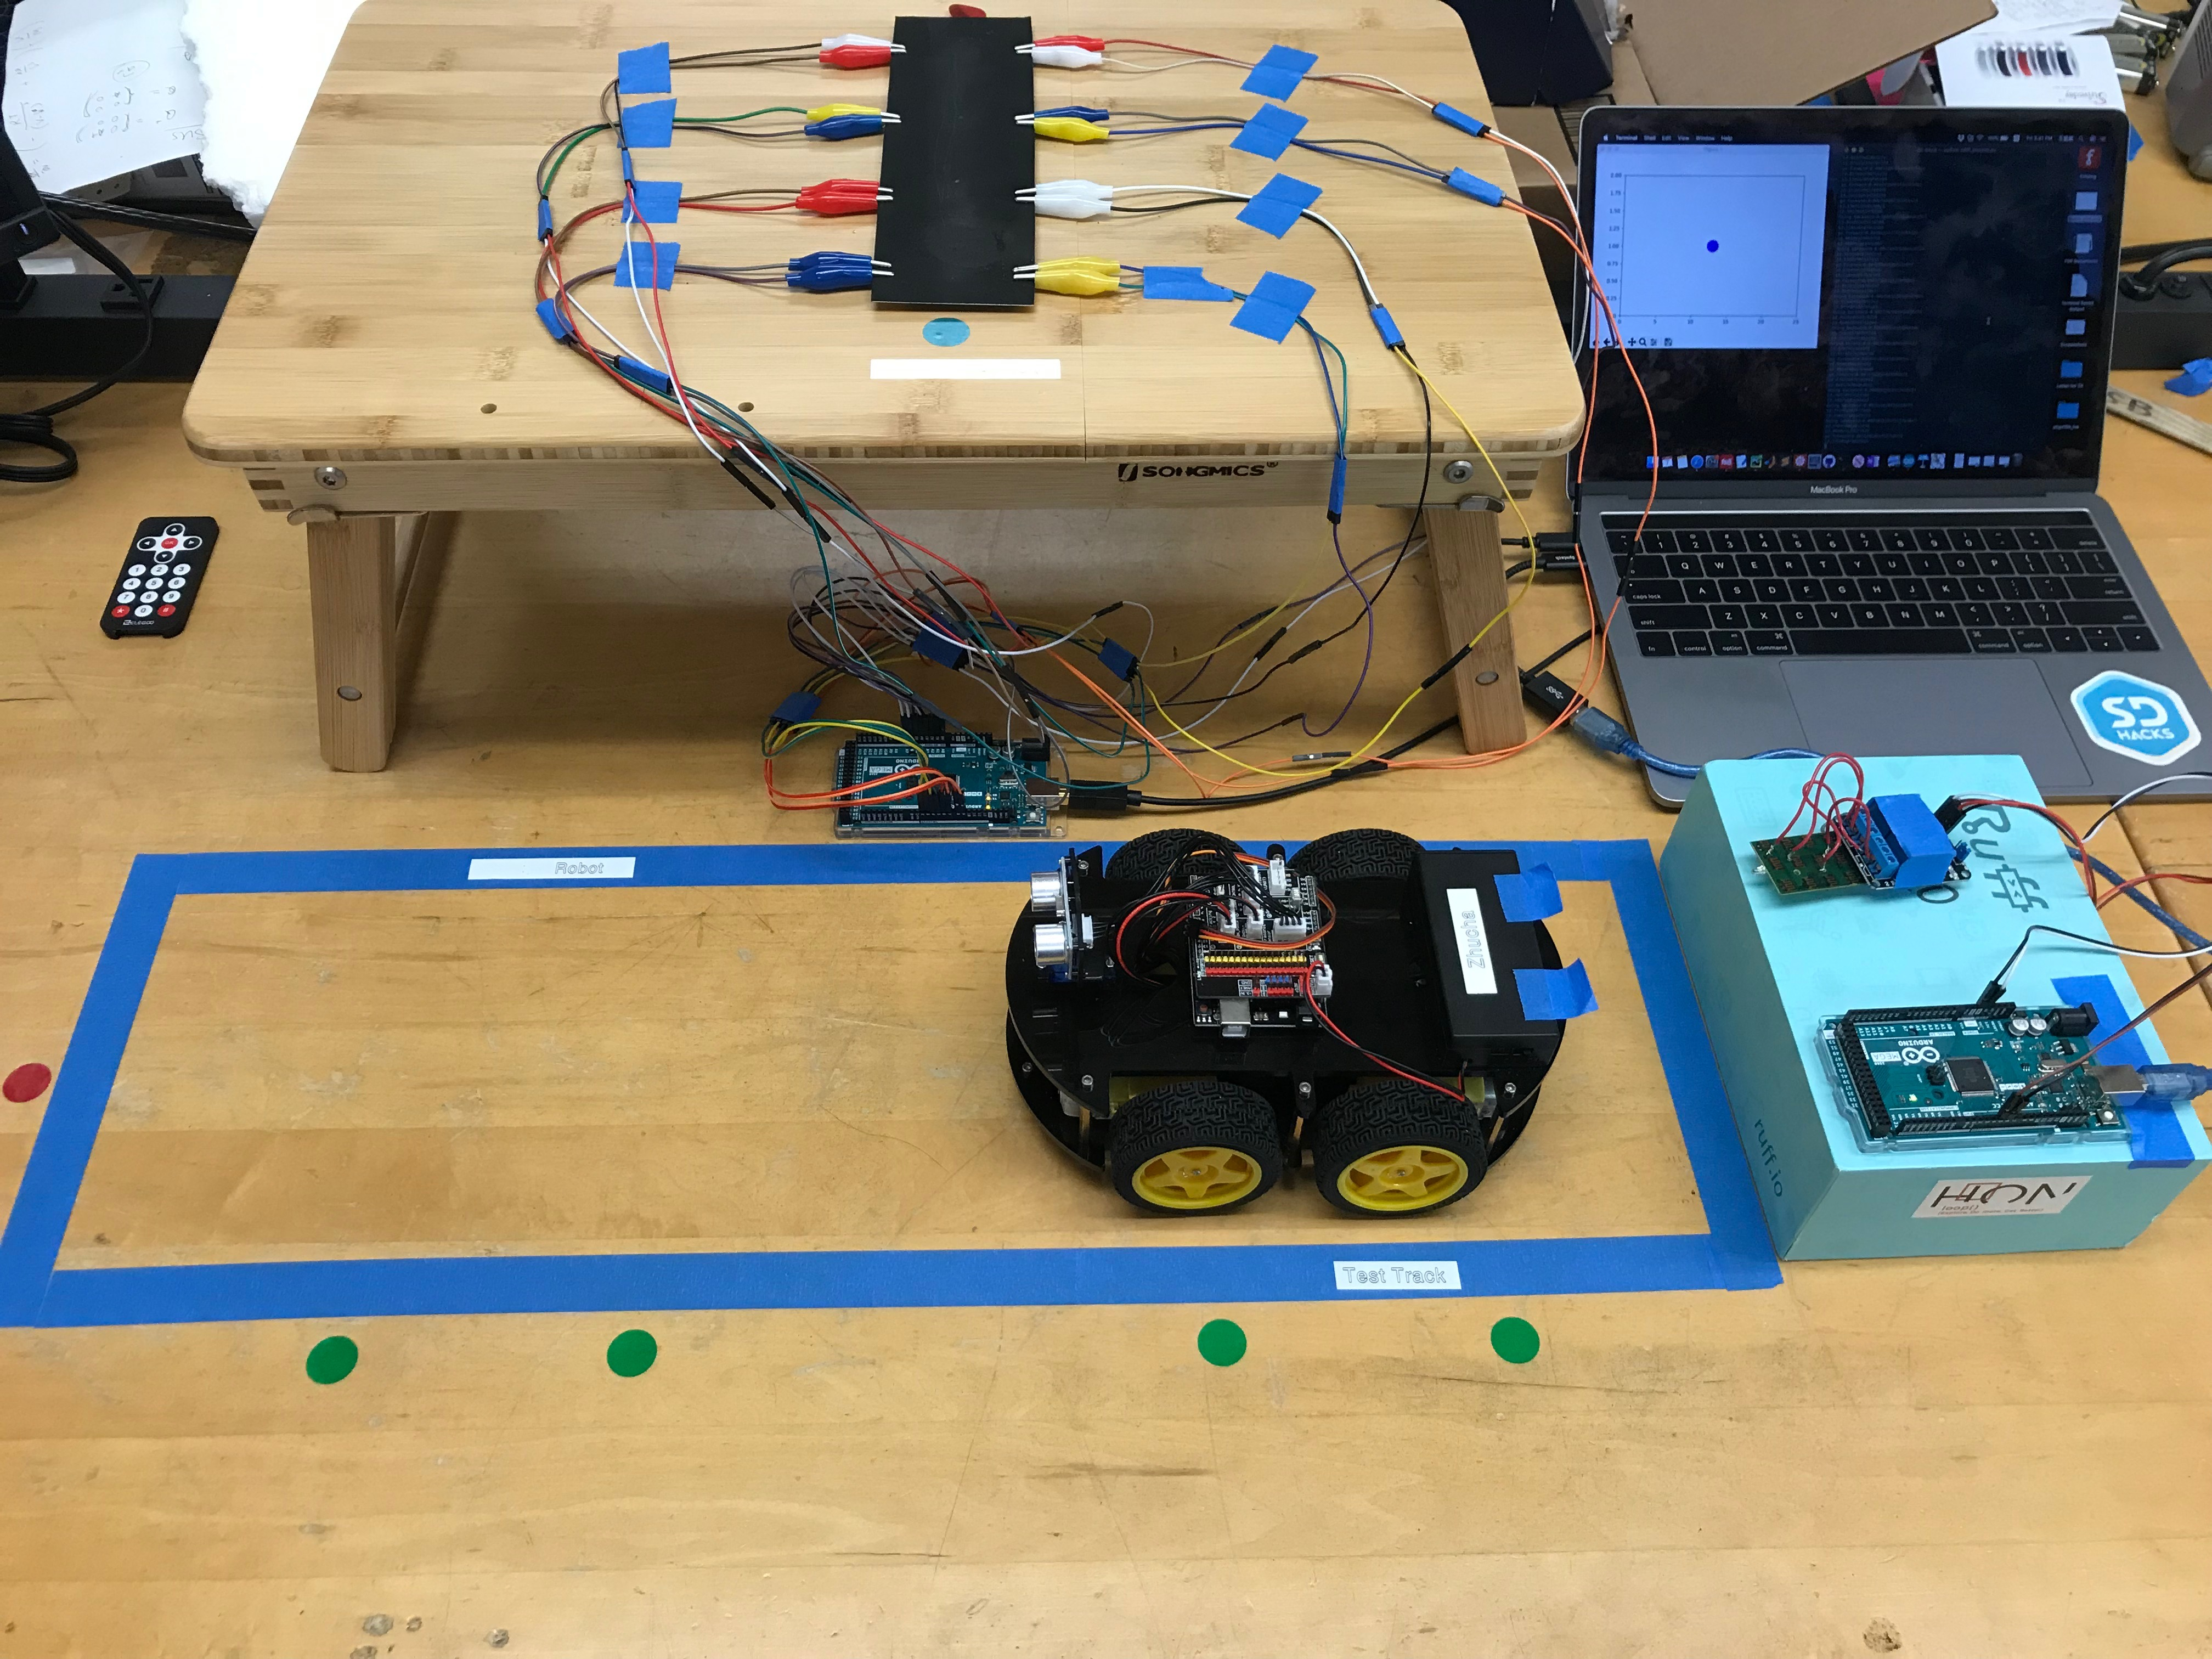
\includegraphics[width=0.4\textwidth]{./figure/setup}     
       \caption{Setup of ROV and touching pad }
    \label{fig::setup}
\end{figure}

\section{Touching Pad}
The goal of the touching pad is that it can be manufactured by shrinking the real size of the actual terrain where the ROV operates. Then, any touching on the touching pad will correspond to a real coordinate in the actual terrain. Therefore, the command applied on the touching pad will correspond to a command of the ROV in the real field. In this section, we are going to introduce the method we constructed the touching pad and the mechanism we use to sense the touch.


\section{Touching Pad}
The goal of the touching pad is that it can be manufactured by shrinking the real size of the actual terrain where the ROV operates. Then, any touching on the touching pad will correspond to a real coordinate in the actual terrain. Therefore, the command applied on the touching pad will correspond to a command of the ROV in the real field. In this section, we are going to introduce the method we constructed the touching pad and the mechanism we use to sense the touch.

\subsection{Electric sensing principle}
Our sensing principle is based on the a carbon-coated plastic board which changes its resistance distribution when the mechanical deformation happens on the board. We also call this method Dynamic Pressure Sensing since as we put our finger on the board, the contact pressure creates the local deformation on the board. This deformation leads to a change in the resistance distribution of the board. 

In Fig. \ref{fig::pressure}, DC current is used to describe the shift of voltage created by the pressing of the finger. When no pressure is applied on the material, the voltage stays constant, which we called baseline. As we may observe, the press of the finger cause an increase of the voltage. When we release the finger, the voltage drops back to the the line which is close to the initial voltage. However, one thing deserved notice is that the voltage does not drop back to the baseline exactly. This phenomenon introduces 3 \% error in this test but we did not consider its effect in our setup of the touching pad. We will discuss the issue in details in the section for future improvement.

\begin{figure}[h]
\centering
    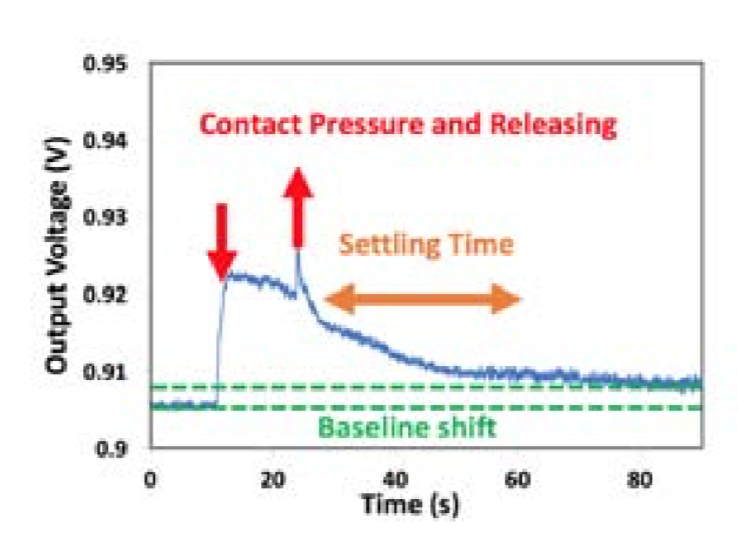
\includegraphics[width=0.45\textwidth]{./figure/pressure}     
       \caption{Voltage reading from a sensing channel fed with fixed DC current upon pressure. The green line (baseline) represent the voltage when no pressure is applied on the board, while the blue line describe the voltage shift caused by the pressing and releasing of the finger. \citep{isoft} }
    \label{fig::pressure}
\end{figure}

In addition, we also tried to implement another popular sensing mechanism based on electric shunting \cite{shunt}, which is implemented by Zhang \cite{electrick}. This mechanism is wildly utilized in Electric Field (EF) sensing systems \cite{ef}. However, this principle requires generating high frequency (200Khz) AC current and higher standard for noise reduction. The wave generator we used, Arduino Mega 2560 \citep{arduino}, cannot generate clean enough signal and the effect of electric shunting cannot be detected from the measurement. Hence, we choose to use the dynamic pressure sensing as our sensing principle.
\subsection{Touching pad setup}
The touching pad is constructed by spraying a conductive carbon paint made by MG Chemicals \citep{carbon} on the surface of a plastic board (25cm $\times$ 6cm). After the spraying, the resistance across the diganol of the board is about 1$\si{k \Omega}$. In Fig. \ref{fig::pad}(a), eight ``electrodes" are placed on the peripheral of the board with separation 6cm and each electrode is consist of 2 alligator clips with one of them applying the voltage and the other measures the voltage. 

\begin{figure}
 	\subfloat[Conductive carbon-coated board with 16 alligator clips. Every 2 alligator clips represent one electrode.]{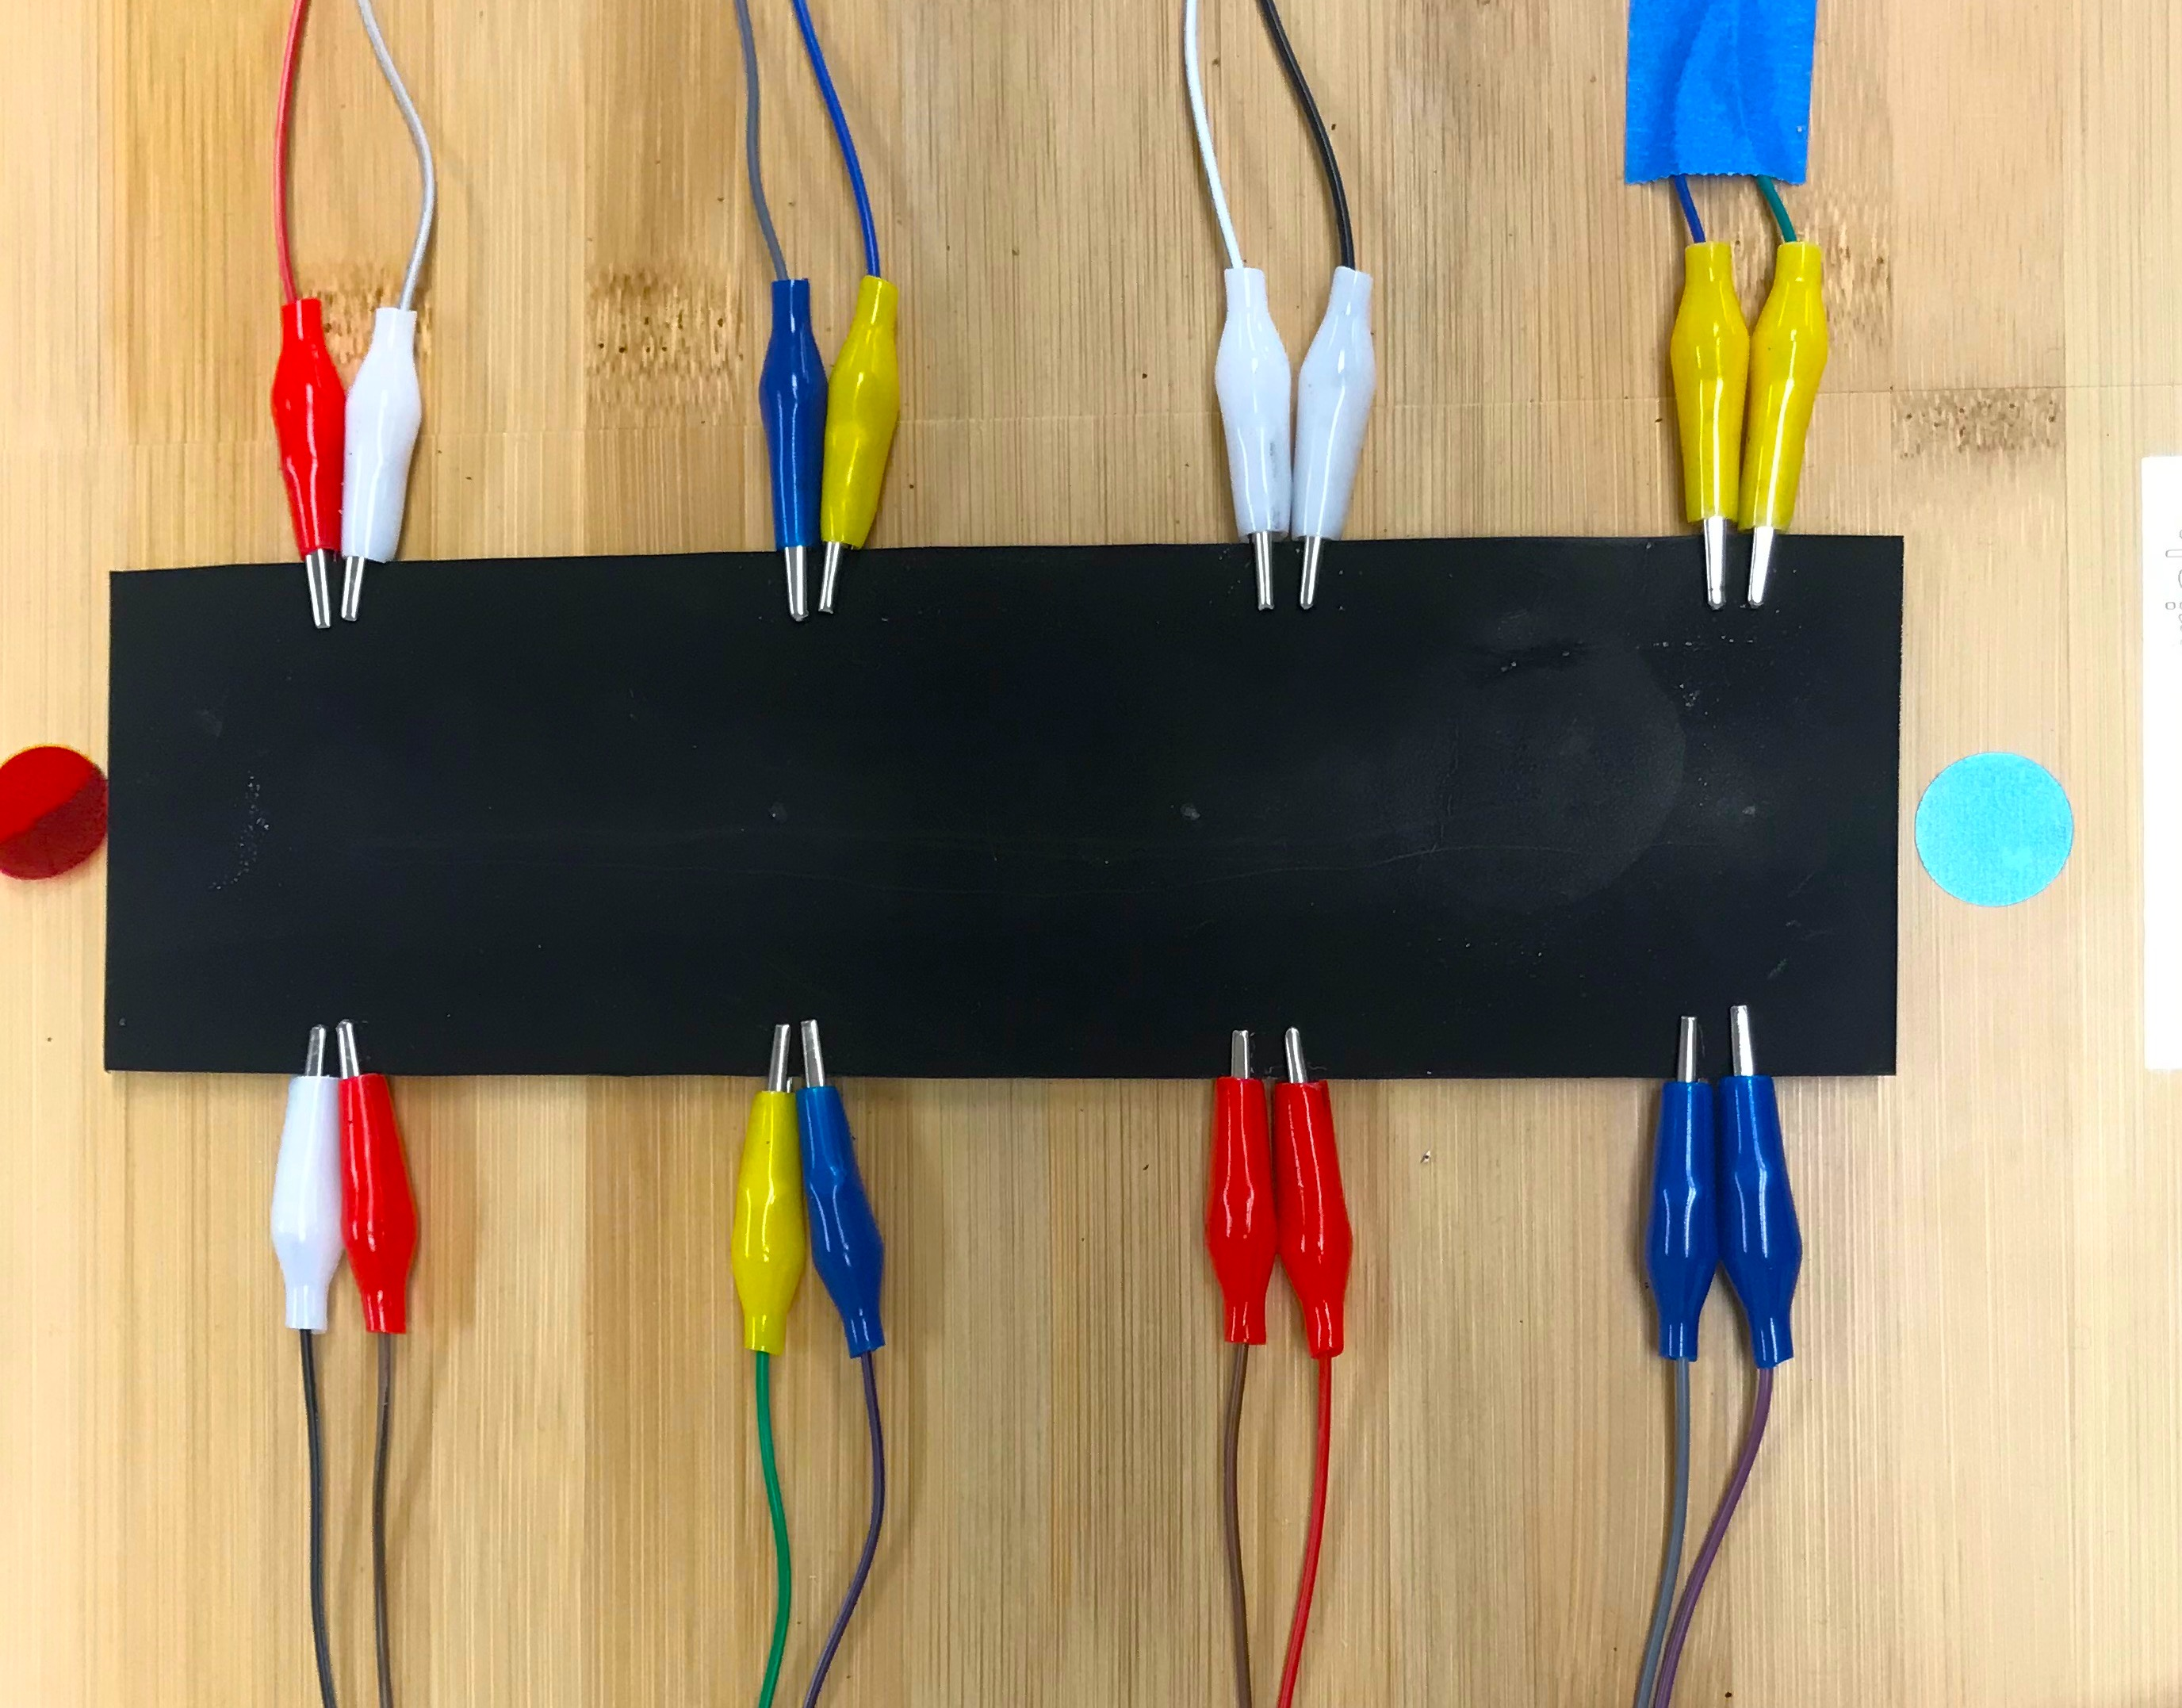
\includegraphics[width=.32\textwidth]{./figure/pad} }\\
 	\subfloat[Schematic diagram with 8 electrodes.]{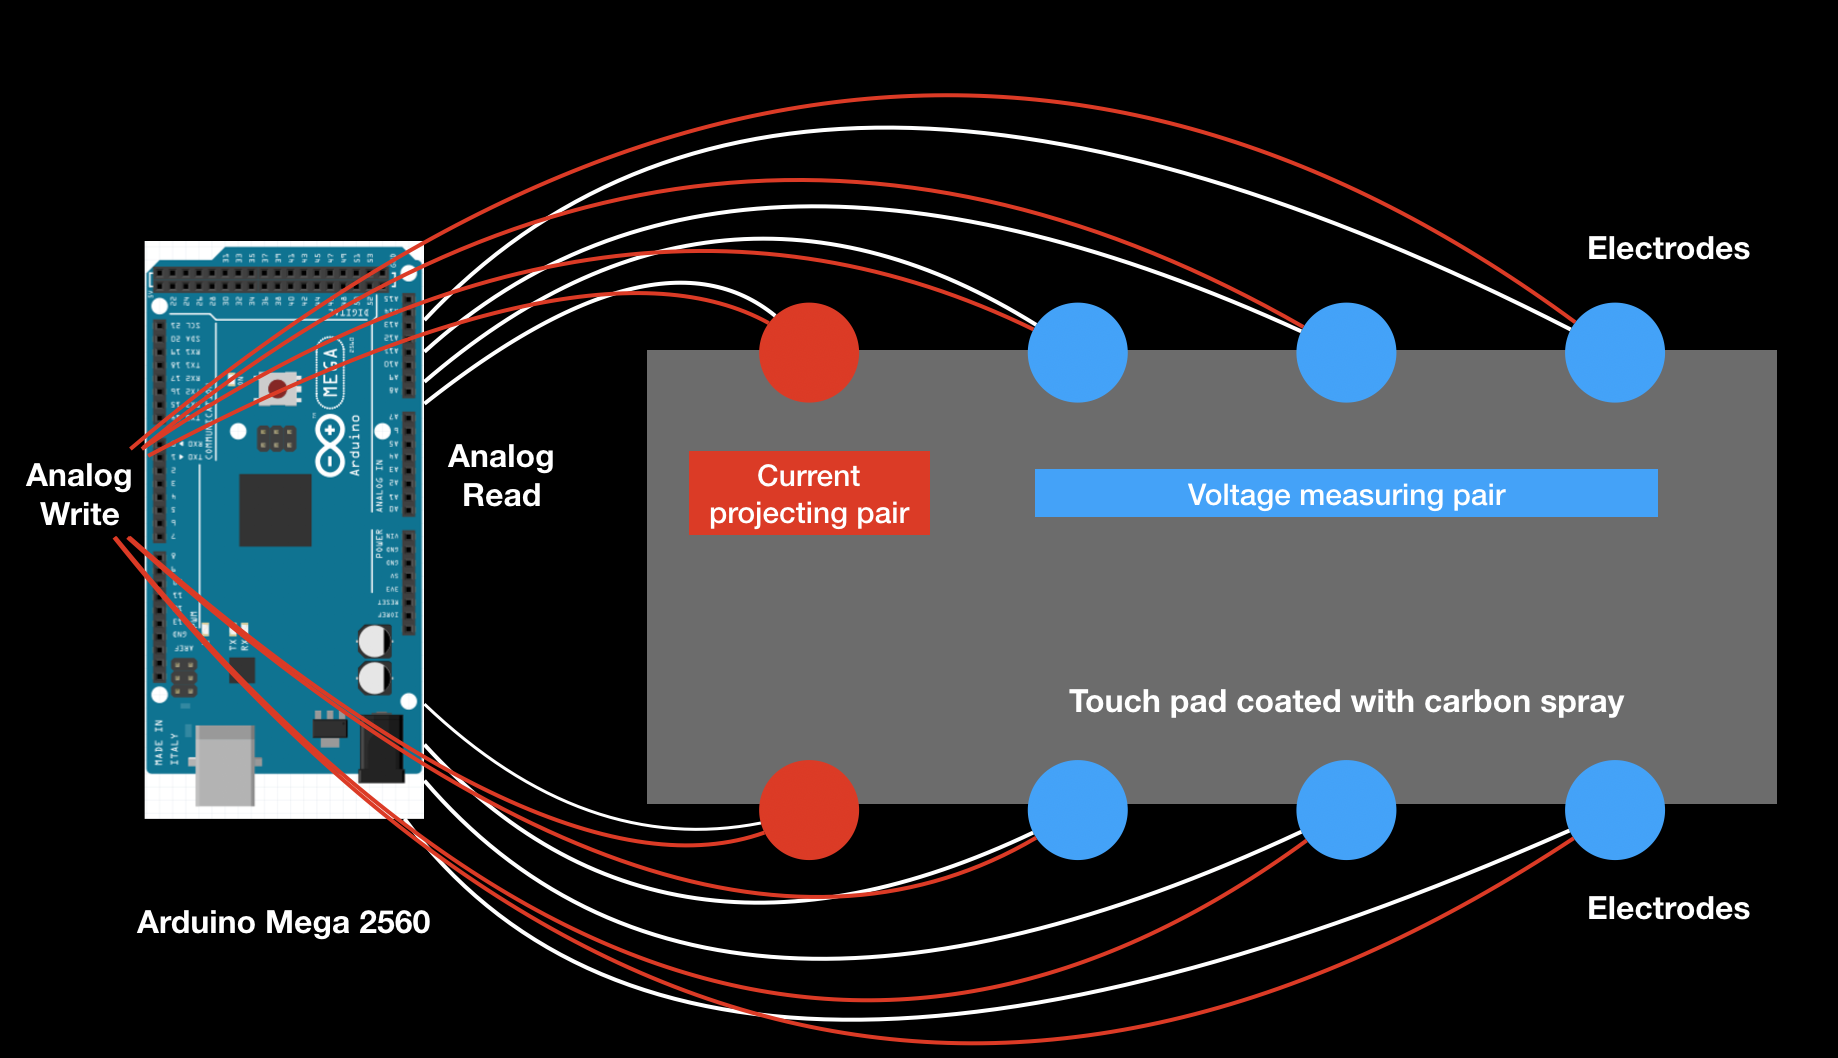
\includegraphics[width=.32\textwidth]{./figure/procedure} } 
\caption{8 electrodes are placed on the peripheral of the touching pad. Every electrode is connect with a Analogwrite pin and Analogread pin.}
 \label{fig::pad}
\end{figure}

\subsection{Measuring procedures}
The measuring procedure requires a pair of electrodes (2 electrodes across the width of the board) to apply a voltage to the touching pad, and we call this pair of electrodes the \textbf{projecting pair}. In the meantime, the other 6 electrodes measure the voltage on each electrode, and we call them \textbf{measuring pair}. Here, we have a projecting pair and three measuring pair and we call this configuration \textbf{1/4 frame}. Then, the projecting pair moves to the right of the previous one. Now, the 2nd pair of electrodes is the projecting pair and the rest becomes the measuring pair. The process iterates until it reaches the most right pair of electrodes. Then, we call we have finished a \textbf{full frame}.

\subsection{Implementation}
In Fig. \ref{fig::pad}(b), the Arduino Mega 2560 applies the voltage in the red pair electrodes. This is realized by setting one electrode 5V and the other 0V, and hence, we will get 5V across the touching pad. Then, the system will delay 100 micro-seconds to stabilize the current. The voltage will be read from the rest of electrodes one by one with reading time 100 micro-seconds for each. Then, we will repeat the reading 40 times, and thus we will have 6 $\times$ 40 = 240 data points from this 1/4 frame. After iterating on the rest 3 pairs, we have 240 $\times$ 4 = 960 data points in total for the full frame. We may calculate the time to acquire the data for the full frame:
\[ 100 \times 4 + 100 \times 960 = 96,400 \text{micro-sec}  = 0.0964 \text{sec},
\]
which is less than 0.1s. We know this is intuitively quite fast.

Then, we have a technical difficulty needs to be resolved when switching the projecting pair to the next. To finish the switch, we should ``close" the previous projecting pair instead of only setting them to 0V. Here, we shall notice the difference between ``close" and grounded. Setting them to 0V basically means that we will have 3 electrodes grounded, and 1 electrode with 5V, which will ruin the configuration. Hence, we need to figure out a way to actually ``close" the electrodes.

The method we find is to set the previous two electrodes to ``INPUT" mode, which set the pin to a high impedance state which has 100 $\si{M\Omega}$. Compared with $1\si{k\Omega}$ of the touching pad, this resistance is enough to let us regard the electrodes as ``close''. This method is efficient since we avoid using a relay, which will tremendously delay our update time for the electric sensing. 


\section{Visualization and Locating Finger}
\subsection{Voltage color-map}
To better monitor the performance of our voltage measurements, we created a real-time voltage map to visualize the data intake at each electrode. In order to see clearly the fluctuations, every time when we run the processing code, we would first run a round of measurement to initialize an offset value that would be subtracted from the later measurements. This is to help us magnify the variations of voltage around a certain value that is different every time due to the easily deformable nature of our touching pad.
\\\indent As we eventually ended using the rectangular touching pad for 1D control, we were aiming for distinguishing the finger locations at four different points. Previously the voltage drop patter could hardly be seen from the voltage map when we attempted to use a large rectangular touching pad. However, as we switched to the 1D touching pad, we could distinguish by eyes that by applying deformation at four different points, we would measure four distinct patterns of voltage drop across the electrodes, as seen in \textbf{Figure  \ref{fig::voltage_map}}.
\begin{figure}
 	\subfloat[]{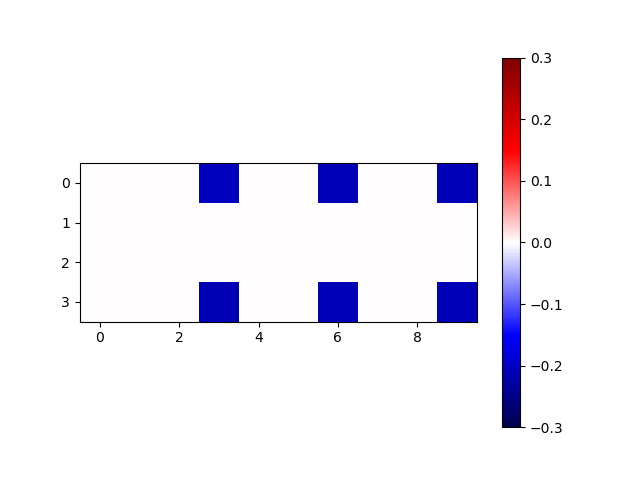
\includegraphics[scale=0.5]{figure/rec1}}\\
 	\subfloat[]{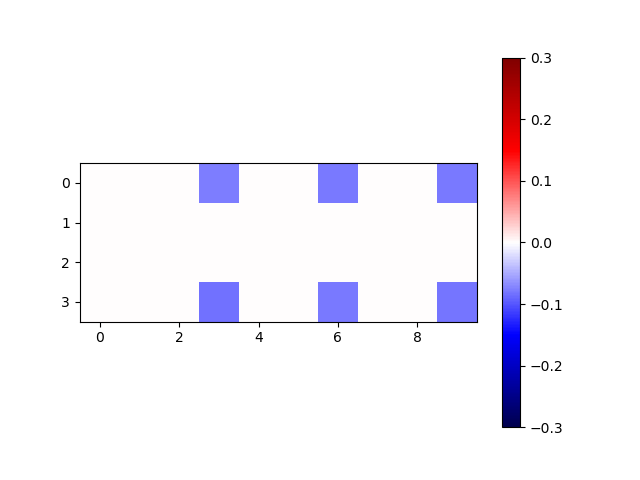
\includegraphics[scale=0.5]{figure/rec2}}\\
 	\subfloat[]{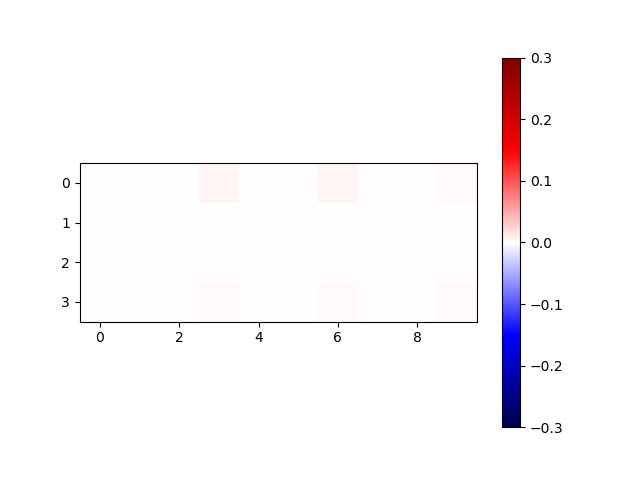
\includegraphics[scale=0.5]{figure/rec3}}\\
 	\subfloat[]{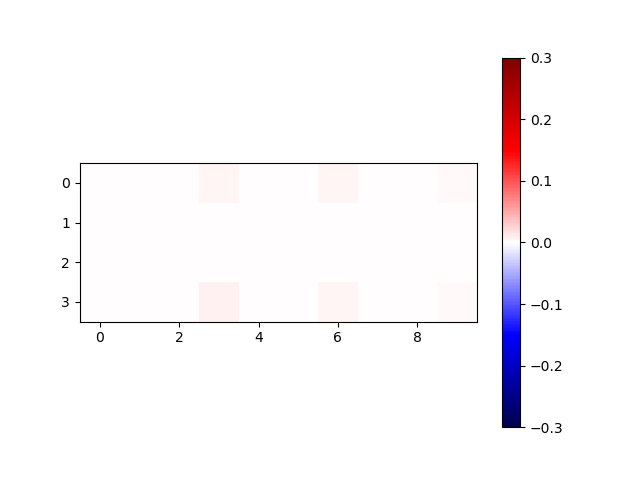
\includegraphics[scale=0.5]{figure/rec4}}
 	\caption{The visualization of voltage measurements when causing deformation at four middle points between opposite electrodes\label{fig::voltage_map}}
\end{figure}
 
\subsection{Locating finger with machine learning}
Originally, we intended to use the electric impedance tomography method to reconstruct the current density over the touching pad. This is a common non-invasive sensing method widely used in medical survey. However, this method only supports still objects that are not subject to deformation, and the most suited situation for using it would be a flat and regularly shaped cross section. Therefore, since our signals come mostly from the deformation of surface, we altered our method to machine learning, which is independent of the various constraint posed by tomography reconstruction.
\\\indent For our machine learning model, we first identify multiple points on the touching pad, and pre-record their coordinates. Then every time when we boot up our program, we would first go through initialization and calibration to train our model. Then using the normal equation (as seen below), we could use this method to predict the finger location.

\begin{equation}
 	\theta = (X^TX)^{-1}(X^Ty)
\end{equation}

In this equation, $\theta$ represents the coefficient for each feature that we used to train our model, each feature being the root mean square of a box of 40 data points we acquired at each electrode; $X$ represent the matrix of the input feature; and $y$ is a column vector that represents the 1D coordinate that corresponds to the voltage feature we recorded in matrix $X$.

\section{Remotely Operated Robot (ROV)}
We assembled our robot using the components that were bought online. We programmed the robot so that it can be controlled by a pre-made infrared remote control. Instead of pushing physical buttons, the remote can be switched on and off by the relay, which is wired to an Arduino Mega connected to the computer. In the graph, the relay and remote is in the lower part connected together by blue tape.

\begin{figure}[!htb]
\begin{center}
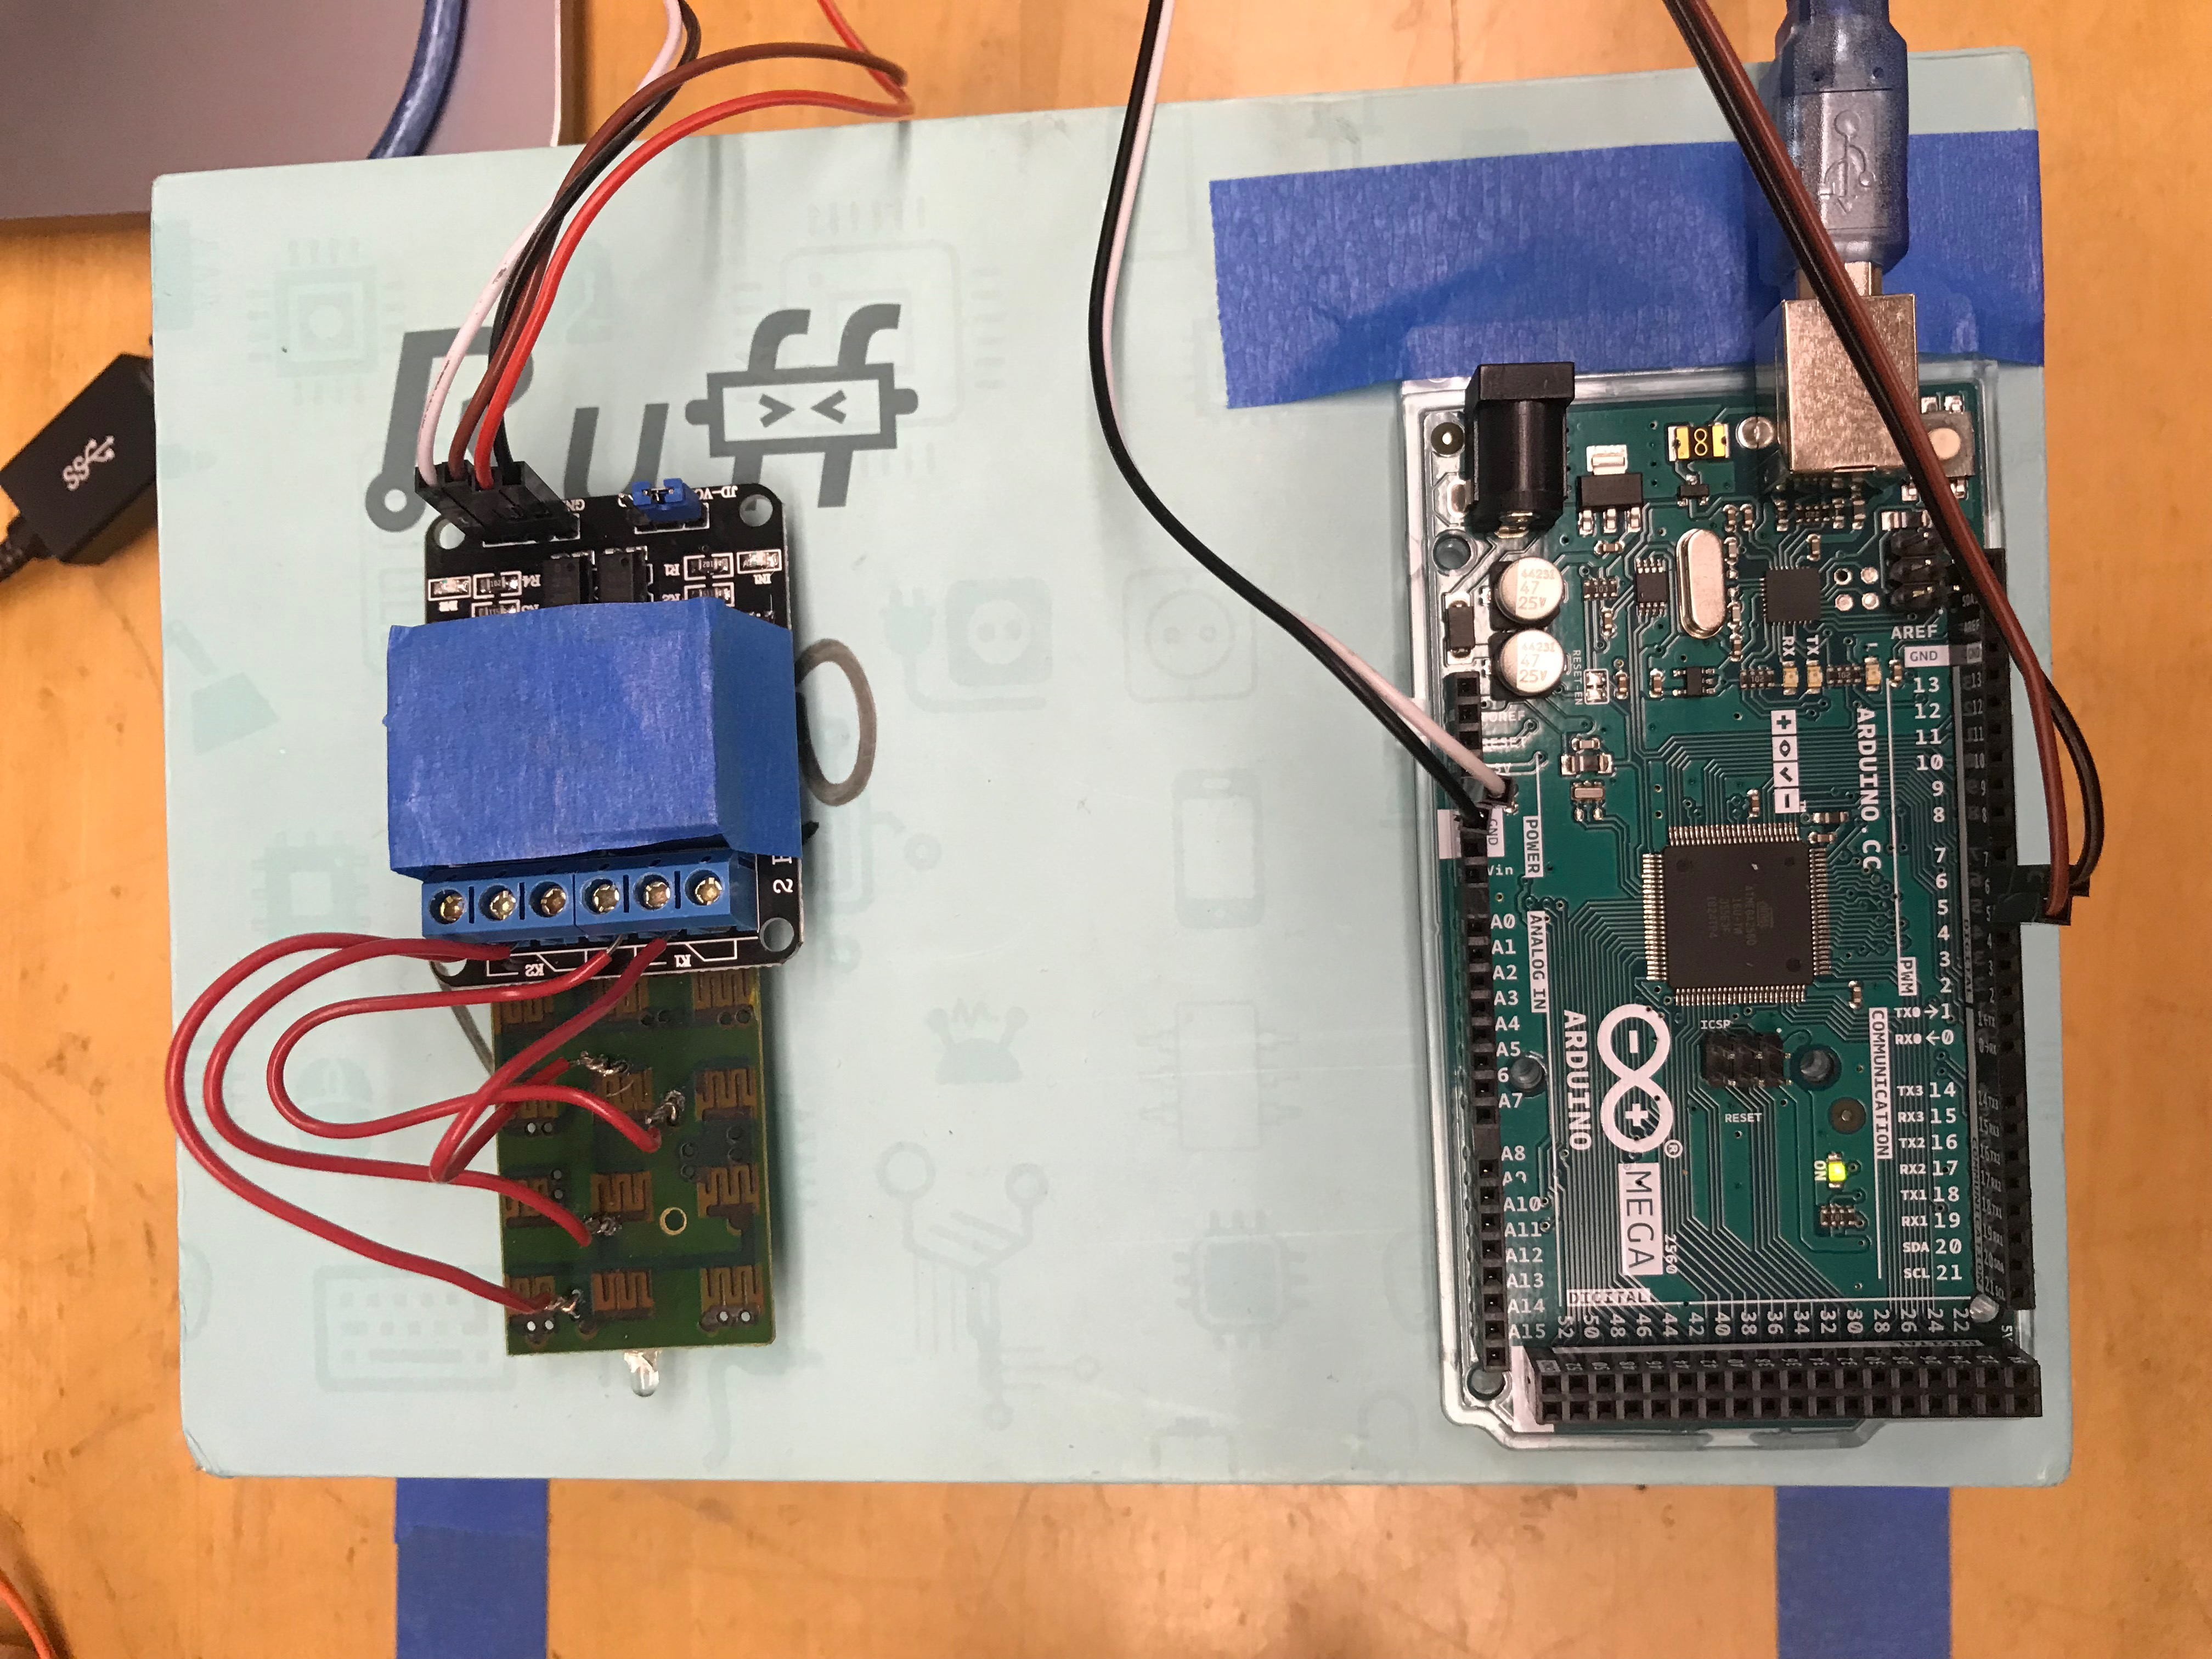
\includegraphics[width=3in]{./figure/relay.jpg}
\caption{Remote control, Relay, and Arduino Mega}
\label{fig1}
\end{center}
\end{figure}

\subsection{Modules}
Our robot is driven by four DC motors. Since we used a L298N dual full bridge driver, the motors of each side had to be wired together. To make the robot move slower, we have gear boxes connected to each of the motors. In addition, PWM is used instead of usual analog pins. We used Arduino Uno to control the whole robot, and mounted Vishley TSOP32238 infrared control on Uno. The power is provided by two 18650 lithium batteries. The robot also comes with other potentially useful components, such as line tracking module, ultrasonic sensor, and bluetooth module.

\subsection{Control method}
Initially we proposed to control the robot using bluetooth module, but after some time, we realized that bluetooth is not a great idea as it is hard to interface with python, not to mention dealing with the various protocols. As a result, we turned to a pre-made remote control instead. We used the relay to control the remote control and the distance robot travels can be monitored by changing the time duration that the remote is switched on. From many trials we found the distance traveled by robot and the remote's ON duration is not a strict linear relationship as we expected. 

As a result, some data is taken and it turns out there was a minimum distance the robot must move. One possible reason is that one complete infrared signal has a minimum required time to send depending on the string that is encoded. In this case, no matter how soon we make the time duration, at a certain point, the signal duration will not become shorter anymore. To resolve this issue, we set the PWM on the motor to the minimum possible (that is, any power lower than this will not be enough to move the robot).Thus, we successfully reduced the minimum distance to about 11.5 centimeters. We also did linear regression to find the correspondence of time and movement distance after minimal distance.

As the accuracy of our track pad is vertainly larger than 1 cm, and the track pad is 23 cm long, we just set the ratio between touch pad and robot movement as 1:11.5 to eliminate the issue. Now this error is acceptable since track pad is now a larger error source.

Some drawbacks of this method is that there is really no feedback, so we were unable to do error control. If we had more time, some possible solutions would be: \\
1) change DC motors into stepper motors, \\
2) build a custom infrared remote so we can directly tell the robot how long to travel, and \\
3) use ultrasonic sensor as a means of feedback.
\subsection{Communication with the touching pad}


\section{Future Improvement}

We used a protocol called pyFirmata to communicate with Arduino from our computer using python. After the individual robot control program is debugged and tested, we integrated it into our main program.
\\\indent For the software part, originally, the machine learning was highly noisy, and the finger location prediction does not provide any sensible data, and we were not able to tell which part went wrong. However, later by measuring 20 sets of data for training the model, we were able to stabilize the resulting finger location on a certain point. And then we were able to recognize the result of our machine learning prediction. At this point, we realized that the prediction was not linear, that is, if we put our finger on four uniformly spaced points, we would get results that has increasing distance between each point. 
\\\indent This turned out to be an issue with the our feature input. We realized that the inputs might not be linearly related to the finger location, and before using the raw data to train our data, an immediate improvement would be to encode it in a different parameter space where the relation between input and finger location is better characterized.

\section{Acknowledgment}
We would like to thank PHYS CS 15C course at UCSB for sponsoring this project, and Prof. Andrew Jayich, Remi Boros, and Craig Holliman for supervising this class.

\nocite{*}
\bibliography{rov}% Produces the bibliography via BibTeX.

\end{document}



